
%(BEGIN_QUESTION)
% Copyright 2015, Tony R. Kuphaldt, released under the Creative Commons Attribution License (v 1.0)
% This means you may do almost anything with this work of mine, so long as you give me proper credit

Sketch connecting wires allowing channel {\tt IN 2} on the data acquisition (DAQ) module to sense the full speed range of the tachogenerator (``tach'') which outputs 0 to 10 volts over a rotational speed range of 0 to 1500 RPM (revolutions per minute).  Feel free to add any additional components you deem necessary to this circuit, as you will need to account for the DAQ's bias current requirements!

\vskip 50pt

$$\includegraphics[width=15.5cm]{i00416x01.eps}$$

\underbar{file i00416}
%(END_QUESTION)





%(BEGIN_ANSWER)

Any solution providing a path for input bias currents to get to the AI Gnd terminal is acceptable.  This may take the form of bias resistors, or simply connecting one of the tachogenerator leads to AI Gnd (either through a resistor to ground or directly to ground):

$$\includegraphics[width=15.5cm]{i00416x02.eps}$$

%(END_ANSWER)





%(BEGIN_NOTES)


%(END_NOTES)


